\chapter{坐标系转换与FlightGear介绍}\label{introduction}
\section{坐标系转换\ucite{4}}
本文这一节主要介绍用于描述飞机姿态位置的坐标系与坐标系之间的转换,用来推导四旋翼飞控建模过程中需要用的旋转矩阵与转换方程。飞机的姿态描述需要利用各种坐标系表示的原因如下:
\begin{enumerate}
	\item 空气动力学的力和力矩是在机体坐标系下表示的。
	\item 牛顿运动方程利用四元数法来表示,需要指明相关的坐标系。
	\item 在机体坐标系下,飞机传感器读取飞机姿态参数信息,比如加速度;相反,飞机上GPS系统读取的飞机位置姿态参数需要在惯性坐标系下(即地面坐标系)。
	\item 大多数情况下,需要在惯性坐标系下,对飞机的飞行轨迹进行描述。另外,地图所采用的位置坐标也是在惯性坐标系下表示的。
\end{enumerate}

要想完成一个坐标系到另一个坐标系之间的转换,需要完成两个步骤,一个是旋转,另一个是转换。在本章的\ref{2.1.1}节部分用来描述坐标旋转矩阵和旋转矩阵应用于坐标系变化;在本章的\ref{2.1.2}节部分用来介绍在四旋翼无人机系统下所采用的特定坐标系,推导四旋翼旋转矩阵表达式;在本章的\ref{2.1.3}节部分用来推导坐标系转换过程中转换关系,即Corlios方程。最终,推导完成坐标系转换过程的两个步骤:旋转和转换。

\subsection{旋转矩阵理论基础}\label{2.1.1}
\begin{figure}[!ht]
\centering
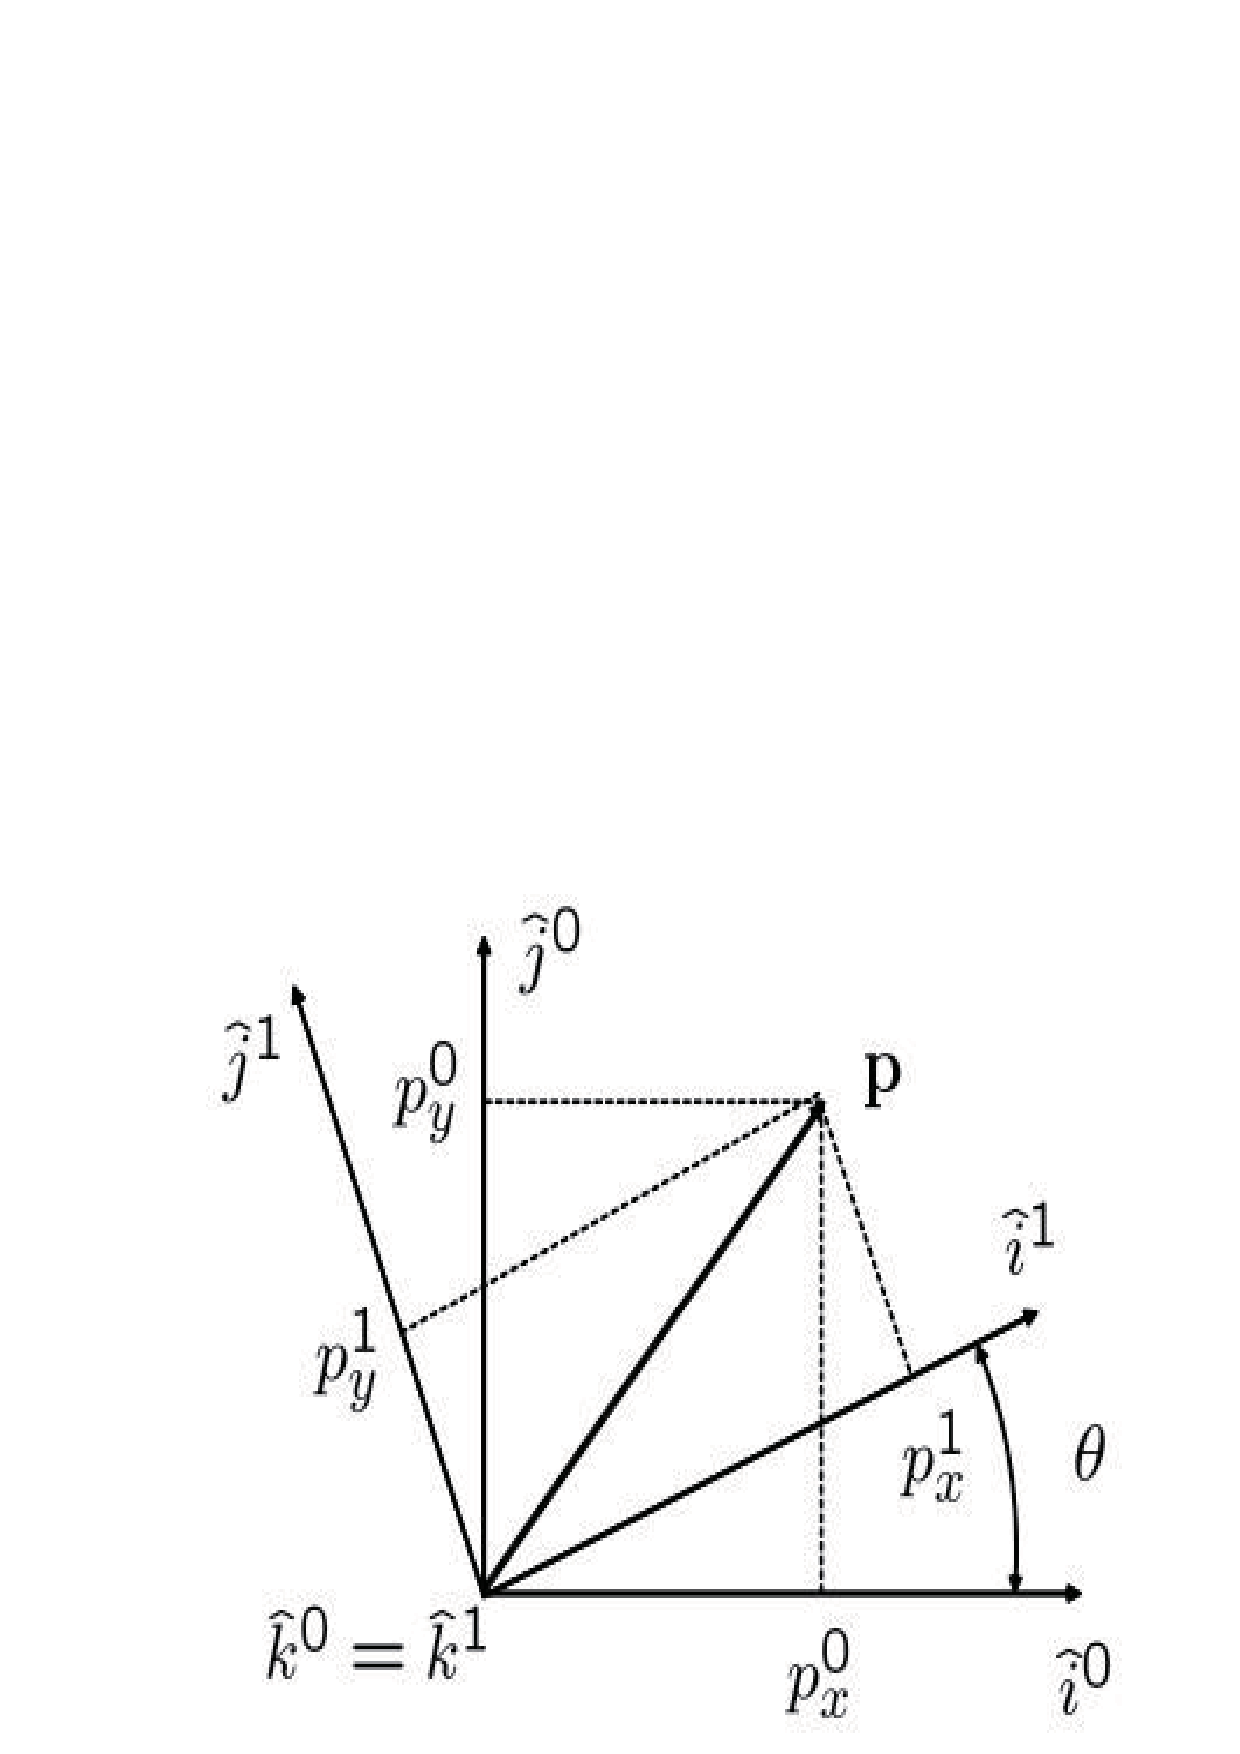
\includegraphics[width=0.6\textwidth]{f2.jpg}
\caption{坐标系二维旋转\ucite{4}}
\label{fig2}
\end{figure}
如图\ref{fig2}所示,向量{\bf{p}}即在坐标系$\mathop R\nolimits^0$下同时还在坐标系$\mathop R\nolimits^1$下,$\mathop R\nolimits^0$坐标系与$\mathop R\nolimits^1$坐标系的坐标原点相同,故向量{\bf{p}}从坐标系$\mathop R\nolimits^0$ 到坐标系$\mathop R\nolimits^1 $的旋转,属于二维空间的旋转。在坐标系$\mathop R\nolimits^0$下,单位向量用$\left( {{{\hat i}^0},{{\hat j}^0},{{\hat k}^0}} \right)$表示,在坐标系$\mathop R\nolimits^1 $下,单位向量用$\left( {{{\hat i}^1},{{\hat j}^1},{{\hat k}^1}} \right)$表示。在坐标系$\mathop R\nolimits^0$下,向量{\bf{p}}可以表示为:
\[\mathop {\bf{p}}\limits^{}  = \mathop p\nolimits_x^0 \mathop {\hat i}\nolimits^0  + \mathop p\nolimits_y^0 \mathop {\hat j}\nolimits^0  + \mathop p\nolimits_z^0 \mathop {\hat k}\nolimits^0 \]

同样,在坐标系系$\mathop R\nolimits^1 $下,向量{\bf{p}}可以表示为:
\[\mathop {\bf{p}}\limits^{}  = \mathop p\nolimits_x^1 \mathop {\hat i}\nolimits^1  + \mathop p\nolimits_y^1 \mathop
{\hat j}\nolimits^1  + \mathop p\nolimits_z^1 \mathop {\hat k}\nolimits^1 \]

联立上面两式,可以得到如下的关系:
\[\mathop p\nolimits_x^0 \mathop {\hat i}\nolimits^0  + \mathop p\nolimits_y^0 \mathop {\hat j}\nolimits^0  + \mathop p\nolimits_z^0 \mathop {\hat k}\nolimits^0  = \mathop p\nolimits_x^1 \mathop {\hat i}\nolimits^1  + \mathop p\nolimits_y^1 \mathop {\hat j}\nolimits^1  + \mathop p\nolimits_z^1 \mathop {\hat k}\nolimits^1 \]

上式两端分别点乘向量$\left( {{{\hat i}^1},{{\hat j}^1},{{\hat k}^1}} \right)$,通过化简可以表示为如下的形式:
\[\mathop {\bf{p}}\nolimits^{\bf{1}} {\kern 1pt} {\kern 1pt} {\kern 1pt} {\kern 1pt}  \buildrel \Delta \over = {\kern 1pt} {\kern 1pt} {\kern 1pt} {\kern 1pt} \left( \begin{array}{l}
\mathop p\nolimits_x^1 \\
\mathop p\nolimits_y^1 \\
\mathop p\nolimits_z^1
\end{array} \right) = \left( {\begin{array}{*{20}{c}}
{\mathop {\hat i}\nolimits^1  \cdot \mathop {\hat i}\nolimits^0 }&{\mathop {\hat i}\nolimits^1  \cdot \mathop {\hat j}\nolimits^0 }&{\mathop {\hat i}\nolimits^1  \cdot \mathop {\hat k}\nolimits^0 }\\
{\mathop {\hat j}\nolimits^1  \cdot \mathop {\hat i}\nolimits^0 }&{\mathop {\hat j}\nolimits^1  \cdot \mathop {\hat j}\nolimits^0 }&{\mathop {\hat j}\nolimits^1  \cdot \mathop {\hat k}\nolimits^0 }\\
{\mathop {\hat k}\nolimits^1  \cdot \mathop {\hat i}\nolimits^0 }&{\mathop {\hat k}\nolimits^1  \cdot \mathop {\hat j}\nolimits^0 }&{\mathop {\hat k}\nolimits^1  \cdot \mathop {\hat k}\nolimits^0 }
\end{array}} \right)\left( \begin{array}{l}
\mathop p\nolimits_x^0 \\
\mathop p\nolimits_y^0 \\
\mathop p\nolimits_z^0
\end{array} \right)\]

通过上式,结合图\ref{fig2}所示的几何关系,可以表示为如下的表达式:
\begin{equation}\label{1}
\mathop {\bf{P}}\nolimits^{\bf{1}}  = \mathop F\nolimits_0^1 \mathop {\bf{P}}\nolimits^{\bf{0}}
\end{equation}

其中,矩阵表示为从坐标系$\mathop R\nolimits^0$到坐标系$\mathop R\nolimits^1$的坐标旋转矩阵,$\theta$ 表示从坐标系$\mathop R\nolimits^0$的$x$轴逆时针旋转到坐标系$\mathop R\nolimits^1$的角度,旋转矩阵$\mathop F\nolimits_0^1 $用$\theta$角来表示,如下所示:
\[\mathop F\nolimits_0^1  = \left( {\begin{array}{*{20}{c}}
{\cos \left( \theta  \right)}&{\sin \left( \theta  \right)}&0\\
{ - \sin \left( \theta  \right)}&{\cos \left( \theta  \right)}&0\\
0&0&1
\end{array}} \right)\]

同理,若坐标系$\mathop R\nolimits^0$的$y$轴,按右手旋转法则转$\theta$角得到坐标系$\mathop R\nolimits^1$,旋转矩阵$\mathop F\nolimits_0^1 $用$\theta$角来表示:
\[\mathop F\nolimits_0^1  \buildrel \Delta \over = \left( {\begin{array}{*{20}{c}}
{\cos \left( \theta  \right)}&0&{ - \sin \left( \theta  \right)}\\
0&1&0\\
{\sin \left( \theta  \right)}&0&{\cos \left( \theta  \right)}
\end{array}} \right)\]

同理,若坐标系$\mathop R\nolimits^0$的$y$轴,按右手旋转法则转$\theta$角得到坐标系$\mathop R\nolimits^1$,旋转矩阵$\mathop F\nolimits_0^1 $用$\theta$角来表示:
\[\mathop F\nolimits_0^1  \buildrel \Delta \over = \left( {\begin{array}{*{20}{c}}
1&0&0\\
0&{\cos \left( \theta  \right)}&{\sin \left( \theta  \right)}\\
0&{ - \sin \left( \theta  \right)}&{\cos \left( \theta  \right)}
\end{array}} \right)\]

通过上面公式,我们可以得到旋转矩阵$\mathop F\nolimits_0^1 $重要的性质,如下所示:
\begin{itemize}
  \item ${\left( {\mathop F\nolimits_a^b } \right)^{{\rm{ - }}1}} = {\left( {\mathop F\nolimits_a^b } \right)^T} = \mathop F\nolimits_a^b $
  \item $\mathop F\nolimits_b^c \mathop F\nolimits_a^b  = \mathop F\nolimits_a^c $
  \item $\det \mathop F\nolimits_a^b  = 1$
\end{itemize}

\begin{figure}[!ht]
\centering
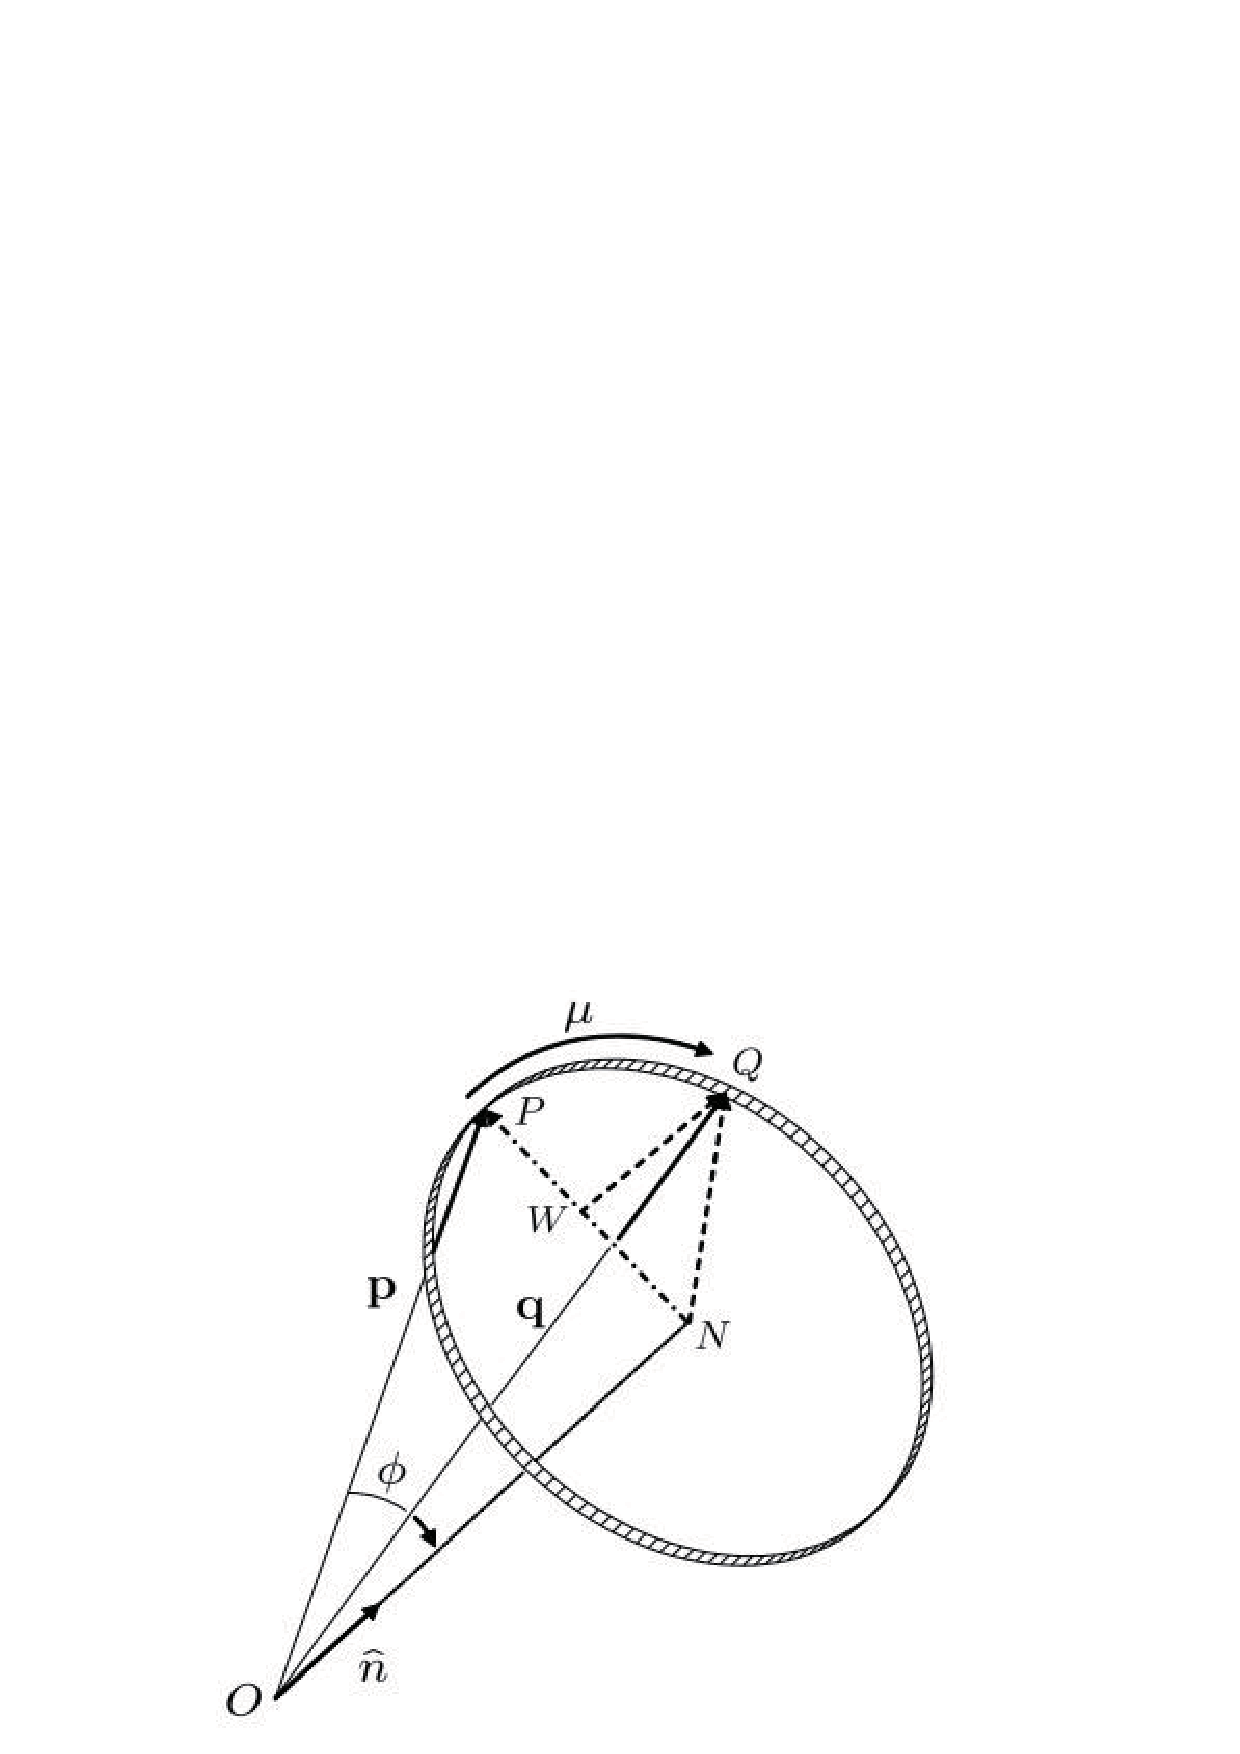
\includegraphics[width=0.6\textwidth]{f3.jpg}
\caption{旋转变换\ucite{4}}
\label{fig3}
\end{figure}

下面我们需要推导旋转公式,采用左手法则,如图\ref{fig3}所示,向量{\bf{p}}顺时针旋转$\mu$得到向量{\bf{q}},$\hat n$ 为单位向量。
\begin{equation}\label{2}
q = O\vec N + N\vec W + W\vec Q
\end{equation}

向量$O\vec N$可以用向量{\bf{p}}和单位向量{\bf{n}}来表示,向量{\bf{p}}在单位向量{\bf{n}}方向投影,得到向量$O\vec N$。
\[O\vec N{\rm{ = }}\left( {{\bf{p}} \cdot \hat n} \right)\hat n\]

向量$N\vec W$方向沿$\vec p - O\vec N$,长度由$NQ\cos \mu $表示。由图\ref{fig3}可知,$NQ$长度与$NP$长度相同,可以用$\left\| {\vec p - \left. {O\vec N} \right\|} \right.$来表示。
\[\begin{array}{l}
\displaystyle{N\vec W{\kern 1pt} {\kern 1pt} {\kern 1pt} {\kern 1pt} {\kern 1pt} {\kern 1pt}  = {\kern 1pt} {\kern 1pt} \frac{{{\bf{p}} - \left( {{\bf{p}} \cdot \hat n} \right)\hat n}}{{\left\| {{\bf{p}} - \left. {\left( {{\bf{p}} \cdot \hat n} \right)\hat n} \right\|} \right.}}}NQ\cos \mu \\
{\kern 1pt} {\kern 1pt} {\kern 1pt} {\kern 1pt} {\kern 1pt} {\kern 1pt} {\kern 1pt} {\kern 1pt} {\kern 1pt} {\kern 1pt} {\kern 1pt} {\kern 1pt} {\kern 1pt} {\kern 1pt} {\kern 1pt} {\kern 1pt} {\kern 1pt} {\kern 1pt} {\kern 1pt} {\kern 1pt} {\kern 1pt} {\kern 1pt} {\kern 1pt} {\kern 1pt} {\kern 1pt} {\kern 1pt} {\kern 1pt} {\kern 1pt} {\kern 1pt} {\kern 1pt} {\kern 1pt} {\kern 1pt} {\kern 1pt} {\rm{ = }}{\kern 1pt} {\kern 1pt} {\kern 1pt} \left( {{\bf{p}} - \left( {{\bf{p}} \cdot \hat n} \right)\hat n} \right)\cos \mu
\end{array}\]

向量$W\vec Q$方向垂直向量{\bf{p}}和{\bf{n}},长度由$NQ\sin \mu $表示。由图\ref{fig3}可知,$NQ$长度也可以用$\left\| {\vec p} \right\|\sin \phi $表示。
\[\begin{array}{l}
\displaystyle{W\vec Q{\kern 1pt} {\kern 1pt} {\kern 1pt} {\kern 1pt} {\rm{ = }}{\kern 1pt} {\kern 1pt} {\kern 1pt} {\kern 1pt} {\kern 1pt} \frac{{{\bf{p}} \times \hat n}}{{\left\| {\bf{p}} \right\|\sin \phi }}}NQ\sin \mu \\
{\kern 1pt} {\kern 1pt} {\kern 1pt} {\kern 1pt} {\kern 1pt} {\kern 1pt} {\kern 1pt} {\kern 1pt} {\kern 1pt} {\kern 1pt} {\kern 1pt} {\kern 1pt} {\kern 1pt} {\kern 1pt} {\kern 1pt} {\kern 1pt} {\kern 1pt} {\kern 1pt} {\kern 1pt} {\kern 1pt} {\kern 1pt} {\kern 1pt} {\kern 1pt} {\kern 1pt}  = {\kern 1pt}  - \hat n \times {\bf{p}}\sin \mu
\end{array}\]
因此,分别将向量$O\vec N$ ,向量$N\vec W$和向量$W\vec Q$表达式代入向量{\bf{q}}的表达式,得到旋转向量表达式,如下所示:
\begin{equation}\label{3}
{\bf{q}} = \left( {1 - \cos \mu } \right)\left( {{\bf{p}} \cdot \hat n} \right)\hat n + \cos \mu {\bf{p}} - \sin \mu \left( {\hat n \times {\bf{p}}} \right)
\end{equation}
\subsection{四旋翼旋转矩阵}\label{2.1.2}
在四旋翼飞行控制时,需要实现不同坐标系之间的转换,下面介绍常用的坐标系。
\subsubsection{惯性坐标系$\mathop R\nolimits^i $}
\begin{figure}[!ht]
\centering
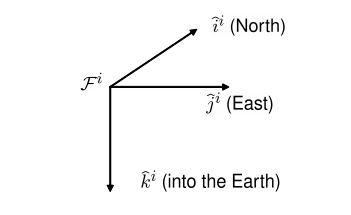
\includegraphics[width=0.4\textwidth]{f5.jpg}
\caption{惯性坐标系\ucite{4}}
\label{fig4}
\end{figure}
惯性坐标系是指坐标原点位于地心,如图\ref{fig4}所示,向量$\hat i$指向北,向量$\hat j$指向东,向量$\hat k$指向地心。
\subsubsection{速度坐标系$\mathop R\nolimits^\nu  $}
\begin{figure}[!ht]
\centering
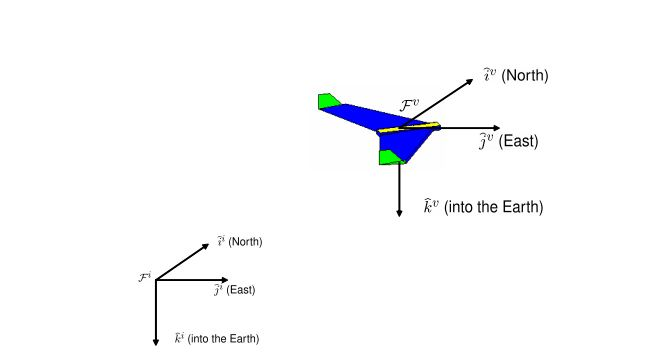
\includegraphics[width=0.9\textwidth]{f6.jpg}
\caption{速度坐标系\ucite{4}}
\label{fig5}
\end{figure}
坐标系的原点位于四旋翼的重心位置,$\mathop R\nolimits^\nu  $坐标系各轴的方向与惯性坐标系$\mathop R\nolimits^i $方向保持一致,如图\ref{fig5}所示。
\subsubsection{偏航坐标系$\mathop R\nolimits^{v1} $}
\begin{figure}[!ht]
\centering
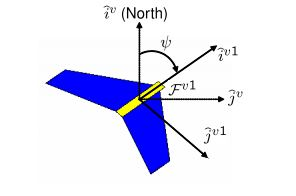
\includegraphics[width=0.6\textwidth]{f7.jpg}
\caption{偏航坐标系\ucite{4}}
\label{fig6}
\end{figure}
$\mathop R\nolimits^{v1} $坐标系的原点位于机体重心位置,$\mathop R\nolimits^{v1} $坐标系是机体绕$\mathop {\hat k}\nolimits^v $轴偏航$\psi $角,从而得到的偏航坐标系,即$\hat i$轴指向机头方向,$\hat j$轴指向右机翼方向,$\hat k$轴指向地心,如图\ref{fig6}所示。

由坐标系$\mathop R\nolimits^v $到坐标系$\mathop R\nolimits^{v1} $的转换,旋转角为$\psi $,利用前面推导的旋转矩阵公式可以得到:
\[\mathop {\bf{p}}\nolimits^{v1}  = \mathop F\nolimits_v^{v1} \left( \psi  \right)\mathop {\bf{p}}\nolimits^v \]

其中,\[\mathop F\nolimits_v^{v1} \left( \psi  \right){\rm{ = }}\left( {\begin{array}{*{20}{c}}
{\cos \psi }&{\sin \psi }&0\\
{ - \sin \psi }&{\cos \psi }&0\\
0&0&1
\end{array}} \right)\]
\subsubsection{俯仰坐标系$\mathop R\nolimits^{v2} $}
\begin{figure}[!ht]
\centering
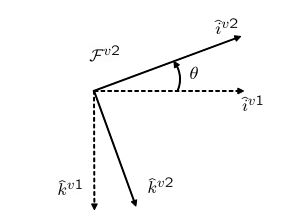
\includegraphics[width=0.6\textwidth]{f8.jpg}
\caption{俯仰坐标系\ucite{4}}
\label{fig7}
\end{figure}
$\mathop R\nolimits^{v2} $坐标系原点位于机体重心位置,$\mathop R\nolimits^{v2} $坐标系是$\mathop R\nolimits^v $坐标系绕$\mathop {\hat j}\nolimits^{v1} $轴俯仰$\theta $角,从而得到的俯仰坐标系,即$\hat i$轴指向机头方向,$\hat j$轴指向右机翼方向,$\hat k$轴指向机身下部。

由坐标系$\mathop R\nolimits^{v1} $到坐标系$\mathop R\nolimits^{v2} $的转换,旋转角为$\theta $,可得:
\[\mathop {\bf{p}}\nolimits^{v2}  = \mathop F\nolimits_{v1}^{v2} \left( \theta  \right)\mathop {\bf{p}}\nolimits^{v1} \]

其中,\[\mathop F\nolimits_{v1}^{v2} \left( \theta  \right) = \left( {\begin{array}{*{20}{c}}
{\cos \theta }&0&{ - \sin \theta }\\
0&1&0\\
{\sin \theta }&0&{\cos \theta }
\end{array}} \right)\]
\subsubsection{机体坐标系$\mathop R\nolimits^b $}
\begin{figure}[!ht]
\centering
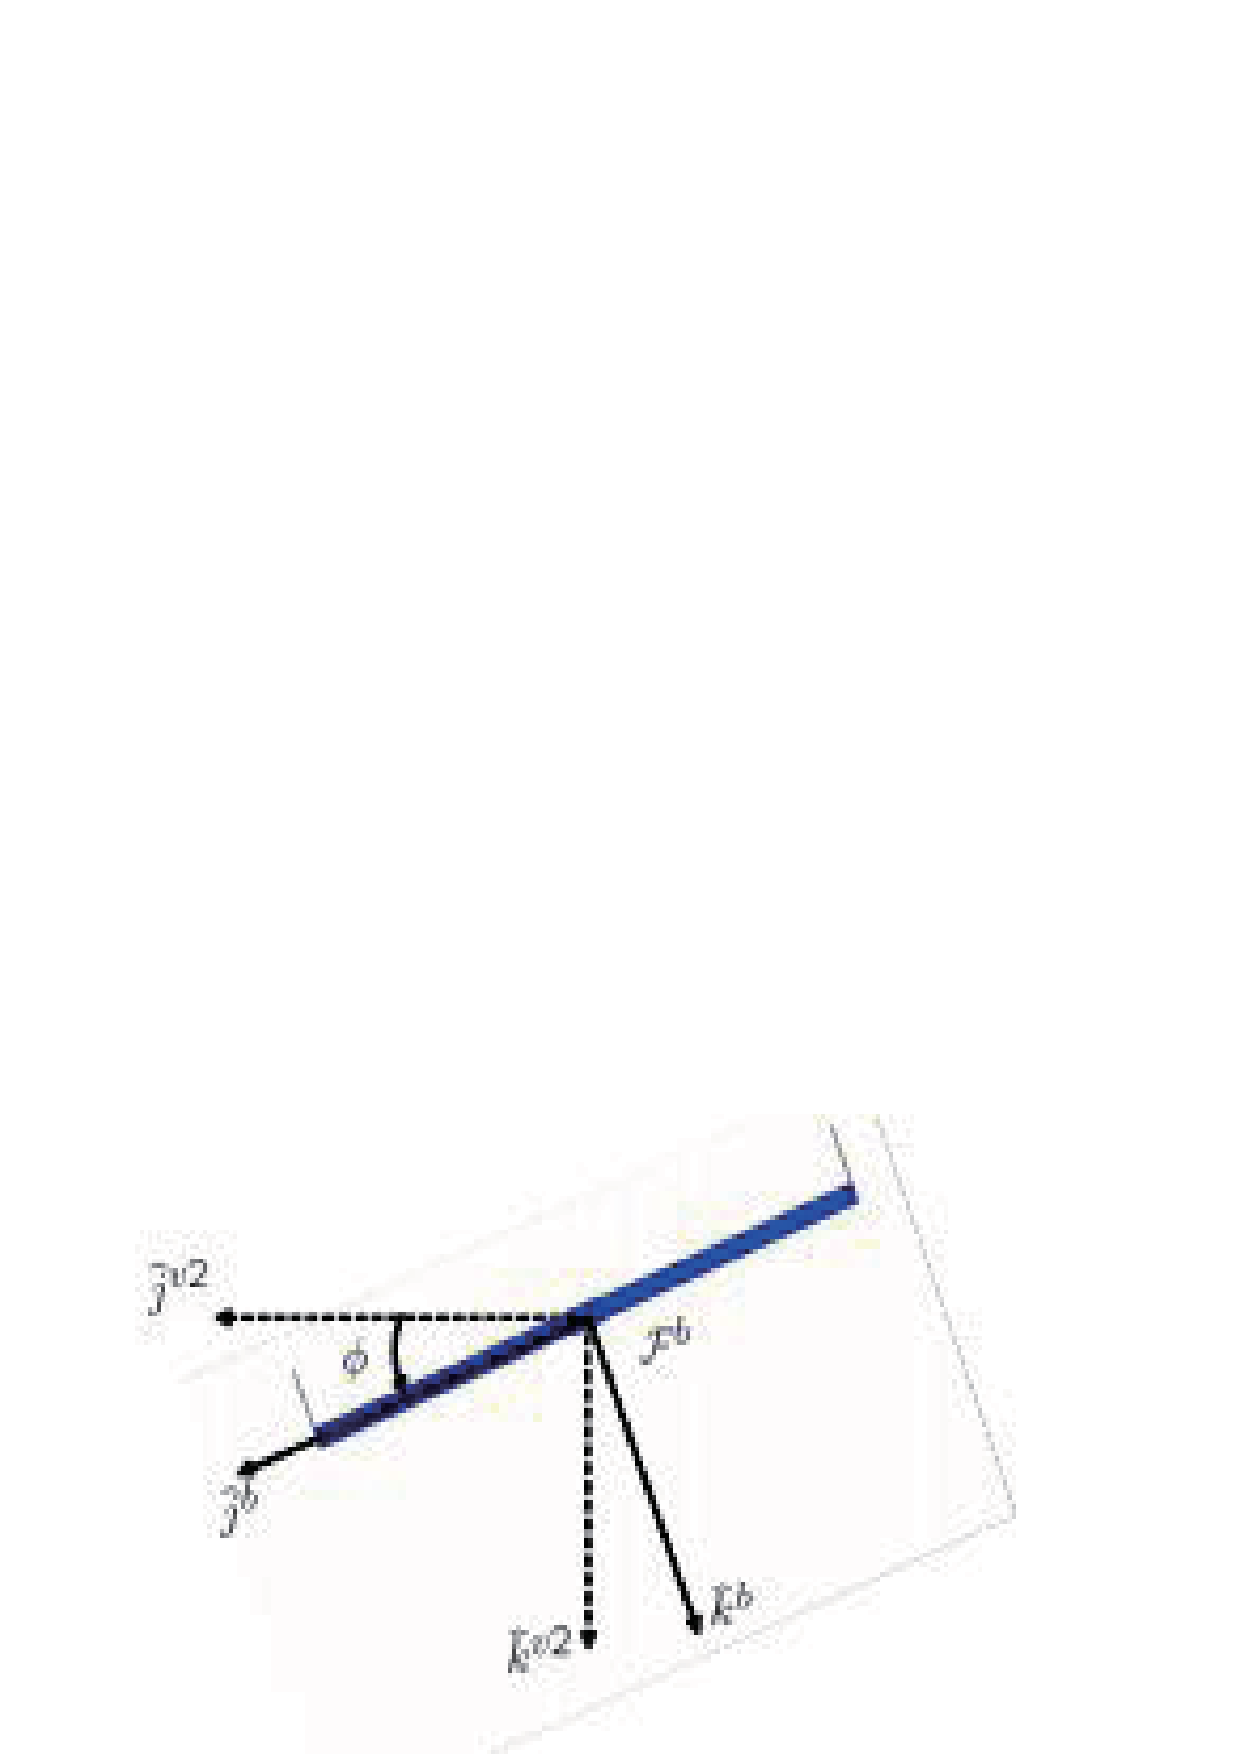
\includegraphics[width=0.6\textwidth]{f9.jpg}
\caption{机体坐标系\ucite{4}}
\label{fig8}
\end{figure}
机体坐标系通过$\mathop R\nolimits^{v2} $绕$\mathop {\hat i}\nolimits^{v2} $轴滚转$\phi $得到$\mathop R\nolimits^b $,如图\ref{fig8}所示。

由坐标系$\mathop R\nolimits^{v2} $到坐标系$\mathop R\nolimits^b $的转换,旋转角为$\phi $ ,可得:
\[\mathop {\bf{p}}\nolimits^b  = \mathop F\nolimits_{v2}^b \left( \phi  \right)\mathop {\bf{p}}\nolimits^{v2} \]

其中,\[\mathop F\nolimits_{v2}^b \left( \phi  \right) = \left( {\begin{array}{*{20}{c}}
1&0&0\\
0&{\cos \phi }&{\sin \phi }\\
0&{ - \sin \phi }&{\cos \phi }
\end{array}} \right)\]

因此,由$\mathop R\nolimits^v $到机体坐标系$\mathop R\nolimits^b $转换,得到的坐标系旋转矩阵。
\[\begin{array}{l}
\mathop F\nolimits_v^b \left( {\phi ,\theta ,\psi } \right) = \mathop F\nolimits_{v2}^b \left( \phi  \right)\mathop F\nolimits_{v1}^{v2} \left( \theta  \right)\mathop F\nolimits_v^{v1} \left( \psi  \right)\\
{\kern 1pt} {\kern 1pt} {\kern 1pt} {\kern 1pt} {\kern 1pt} {\kern 1pt} {\kern 1pt} {\kern 1pt} {\kern 1pt} {\kern 1pt} {\kern 1pt} {\kern 1pt} {\kern 1pt} {\kern 1pt} {\kern 1pt} {\kern 1pt} {\kern 1pt} {\kern 1pt} {\kern 1pt} {\kern 1pt} {\kern 1pt} {\kern 1pt} {\kern 1pt} {\kern 1pt} {\kern 1pt} {\kern 1pt} {\kern 1pt} {\kern 1pt} {\kern 1pt} {\kern 1pt} {\kern 1pt} {\kern 1pt} {\kern 1pt} {\kern 1pt} {\kern 1pt} {\kern 1pt} {\kern 1pt} {\kern 1pt} {\kern 1pt} {\kern 1pt} {\kern 1pt} {\kern 1pt} {\kern 1pt} {\kern 1pt} {\kern 1pt} {\kern 1pt} {\kern 1pt} {\kern 1pt} {\kern 1pt} {\kern 1pt} {\kern 1pt} {\kern 1pt} {\kern 1pt} {\kern 1pt} {\kern 1pt} {\kern 1pt} {\kern 1pt} {\kern 1pt}  = \left( {\begin{array}{*{20}{c}}
1&0&0\\
0&{\cos \phi }&{\sin \phi }\\
0&{ - \sin \phi }&{\cos \phi }
\end{array}} \right)\left( {\begin{array}{*{20}{c}}
{\cos \theta }&0&{ - \sin \theta }\\
0&1&0\\
{\sin \theta }&0&{\cos \theta }
\end{array}} \right)\left( {\begin{array}{*{20}{c}}
{\cos \psi }&{\sin \psi }&0\\
{ - \sin \psi }&{\cos \psi }&0\\
0&0&1
\end{array}} \right)\\
{\kern 1pt} {\kern 1pt} {\kern 1pt} {\kern 1pt} {\kern 1pt} {\kern 1pt} {\kern 1pt} {\kern 1pt} {\kern 1pt} {\kern 1pt} {\kern 1pt} {\kern 1pt} {\kern 1pt} {\kern 1pt} {\kern 1pt} {\kern 1pt} {\kern 1pt} {\kern 1pt} {\kern 1pt} {\kern 1pt} {\kern 1pt} {\kern 1pt} {\kern 1pt} {\kern 1pt} {\kern 1pt} {\kern 1pt} {\kern 1pt} {\kern 1pt} {\kern 1pt} {\kern 1pt} {\kern 1pt} {\kern 1pt} {\kern 1pt} {\kern 1pt} {\kern 1pt} {\kern 1pt} {\kern 1pt} {\kern 1pt} {\kern 1pt} {\kern 1pt} {\kern 1pt} {\kern 1pt} {\kern 1pt} {\kern 1pt} {\kern 1pt} {\kern 1pt} {\kern 1pt} {\kern 1pt} {\kern 1pt} {\kern 1pt} {\kern 1pt} {\kern 1pt} {\kern 1pt} {\kern 1pt} {\kern 1pt} {\kern 1pt} {\kern 1pt} {\kern 1pt} {\rm{ = }}\left( {\begin{array}{*{20}{c}}
{c\theta c\psi }&{c\theta s\psi }&{ - s\theta }\\
{s\phi s\theta c\psi  - c\phi s\psi }&{s\phi s\theta s\psi  + c\phi c\psi }&{s\phi c\theta }\\
{c\phi s\theta c\psi  + s\phi s\psi }&{c\phi s\theta s\psi  - s\phi c\psi }&{c\psi c\theta }
\end{array}} \right)
\end{array}\]

其中,$c\phi  \buildrel \Delta \over = \cos \phi $,$s\phi  \buildrel \Delta \over = \sin \phi $。
\subsection{Coriolis公式}\label{2.1.3}
在这一节,本文打算推导Coriolis数学关系式为后面飞控动力学关系作铺垫,Coriolis公式在坐标系变换过程中,起到非常重要的作用。假设,我们有两个坐标系,机体坐标系$\mathop R\nolimits^b $和惯性坐标系$\mathop R\nolimits^i $,如图\ref{fig9} 所示,向量${\bf{p}}$相对坐标系$\mathop R\nolimits^i $的运动,可以分解为两个运动,即:有向量${\bf{p}}$ 随着机体坐标系$\mathop R\nolimits^b $的平动,和向量${\bf{p}}$相对$\mathop R\nolimits^i $ 坐标系转动。
\begin{figure}[!ht]
\centering
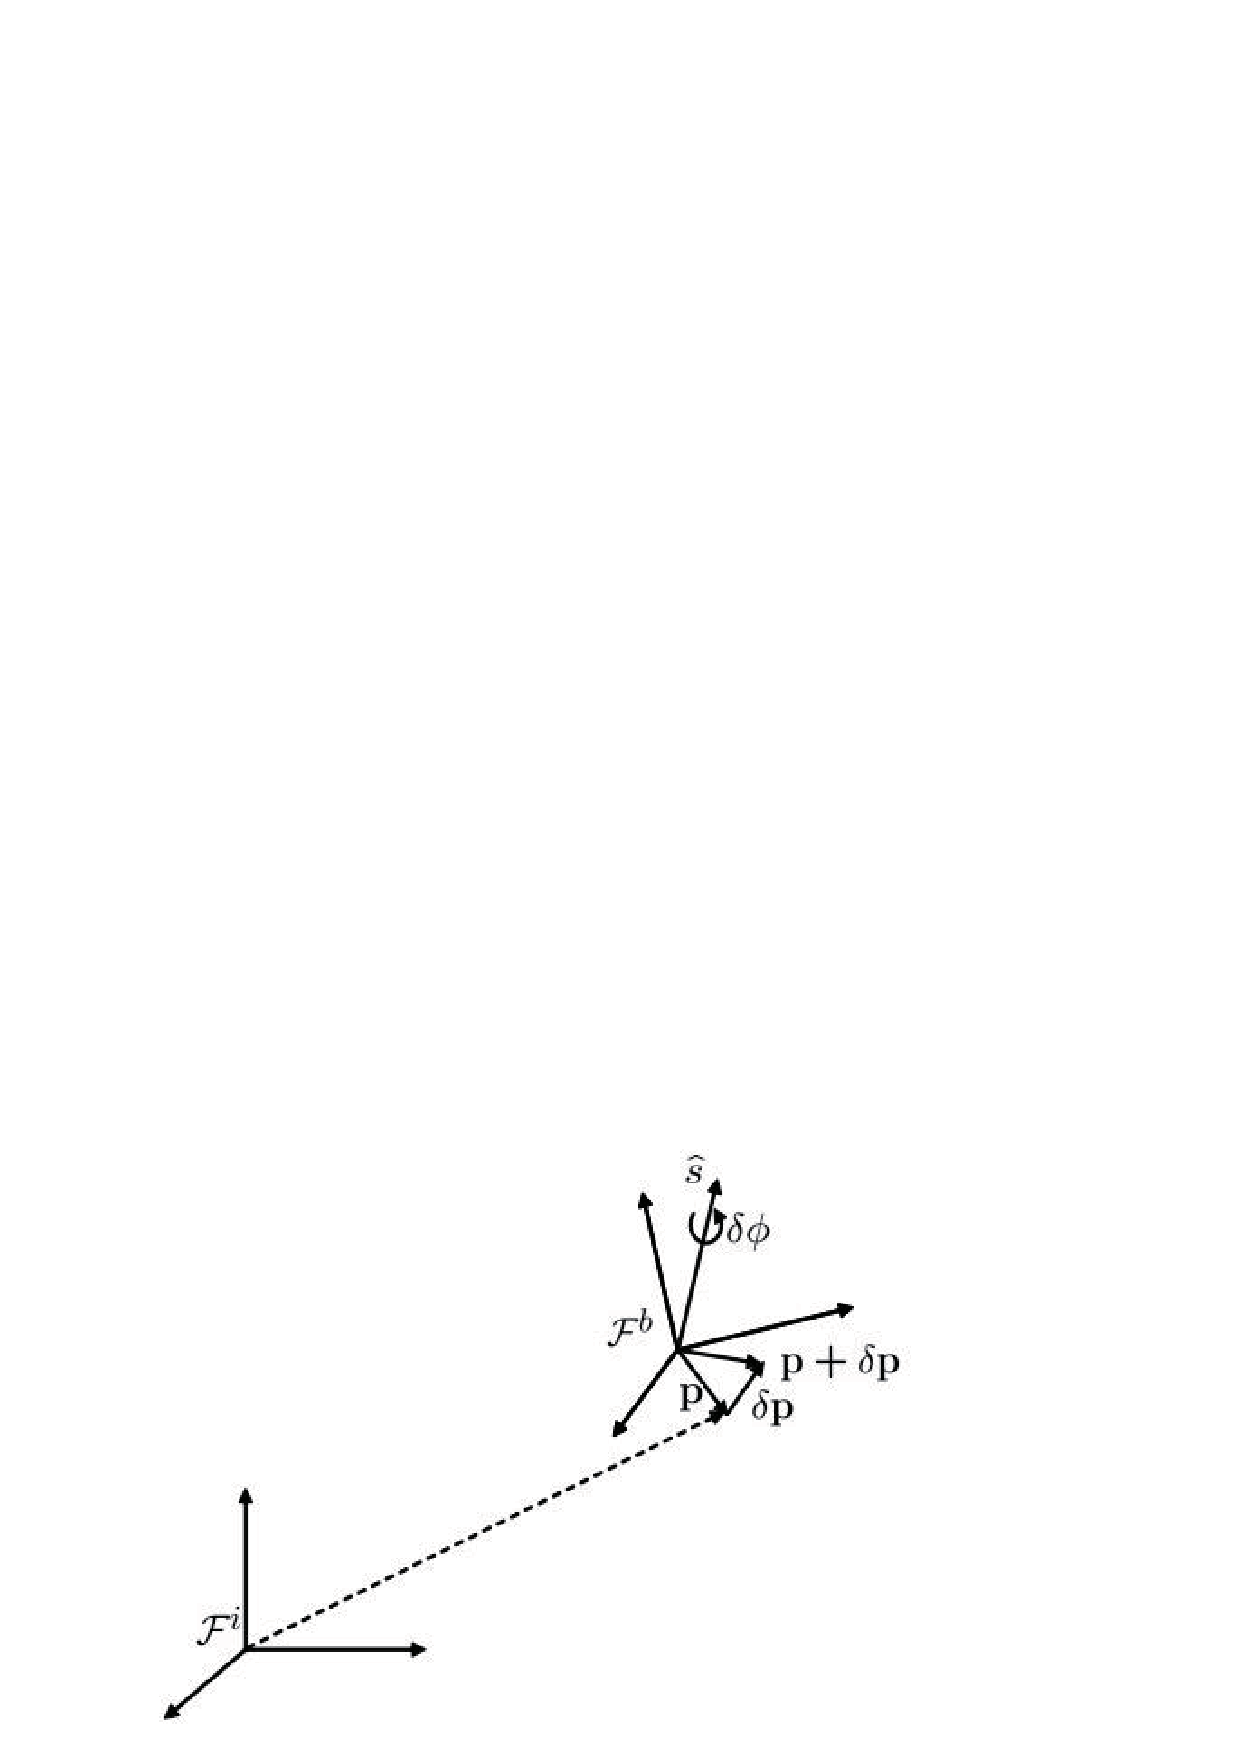
\includegraphics[width=0.6\textwidth]{f10.jpg}
\caption{Coriolis公式推导图\ucite{4}}
\label{fig9}
\end{figure}
下面总共两步推导Coriolis公式\ucite{15}:

\textbf{Step1:}

首先,假设机体坐标系$\mathop R\nolimits^b $不相对惯性坐标系$\mathop R\nolimits^i $转动,向量${\bf{p}}$随着向量机体坐标系$\mathop R\nolimits^b $ 平动,向量${\bf{p}}$相对惯性坐标系$\mathop R\nolimits^i $运动等价于向量${\bf{p}}$ 相对机体坐标系$\mathop R\nolimits^b $ 运动,如下所示:
\begin{equation}\label{4}
\frac{d}{{d{t_i}}}{\bf{p}} = \frac{d}{{d{t_b}}}{\bf{p}}
\end{equation}

\textbf{Step2:}

向量${\bf{p}}$静止在坐标系$\mathop R\nolimits^b $内,同时,坐标系$\mathop R\nolimits^b $相对坐标系$\mathop R\nolimits^i $ 转动,因此,向量${\bf{p}}$相对$\mathop R\nolimits^i $ 坐标系转动等效于坐标系$\mathop R\nolimits^b $相对坐标系$\mathop R\nolimits^i $转动,利用前面推导的旋转公式\ref{3},可得如下关系:
\[\vec p + \delta \vec p = \left( {1 - \cos \left( { - \delta \phi } \right)} \right)\hat s\left( {\hat s \cdot \vec p} \right) + \cos \left( { - \delta \phi } \right)\vec p - \sin \left( { - \delta \phi } \right)\hat s \times \vec p\]

利用小角度近似,同时等式两边同时除以$\delta t$,可得如下关系:
\[\frac{{\delta p}}{{\delta t}} \approx \frac{{\delta \phi }}{{\delta t}} \times \vec p\]

当$\delta t \to 0$时,$\mathop R\nolimits^b $坐标系相对$\mathop R\nolimits^i$坐标系的角速度可以表示为:${\omega _{b/i}} \buildrel \Delta \over = \hat s\dot \phi $,代入上式可得:
\begin{equation}\label{5}
{\frac{d}{{dt}}_i}{\bf{p}} = {\omega _{b/i}} \times {\bf{p}}
\end{equation}

因为,微分方程的线性性质,可以将公式\ref{4}和公式\ref{5}线性相加,便可得到Coriolis方程:
\begin{equation}
\frac{d}{{d{t_i}}}{\bf{p}} = \frac{d}{{d{t_b}}}{\bf{p}} + {\omega _{b/i}} \times {\bf{p}}
\end{equation}
\section{FlightGear软件介绍}
FlightGear是一个开源的飞行器模拟软件,由飞行模拟爱好者和编程爱好者共同合作开发的一款通过互联网提供大家学习的软件。FlightGear开发的原因一方面因为商业的飞行模拟软件价格高,受众群体小;另一方面,大多数商业的飞行模拟软件由于研发资金与开发时间的限制,并不能够提供一款功能全面的逼真的飞行模拟软件\ucite{8}。

\begin{figure}[!ht]
\centering
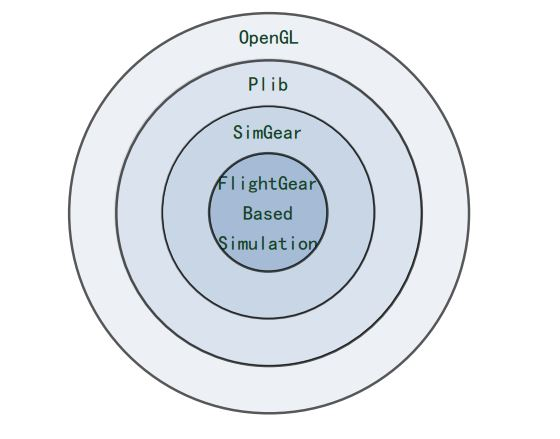
\includegraphics[width=0.5\textwidth]{f20.jpg}
\caption{FlightGear主要组件\ucite{9}}
\label{fig10}
\end{figure}
FlightGear作为一款大型的飞行模拟软件,结合了许多轻量级的开源软件。FlightGear主要使用的软件之间的关系如图\ref{fig10} 所示。下面分别介绍OpenGL, Plib和SimGear 在FlightGear功能实现过程中的功能与作用。
\begin{itemize}
  \item OpenGL

  OpenGL 是 Open Graphics Library 的缩写,意为开放的图形库,是 FlightGear最重要的组件。它是 SGI 公司开发的基于 FlightGear 的直升机飞行模拟系统研究的一套高性能图形处理系统,GL 代表图形库(Graphics  Library),前身是 SGI的 IRIX GL(工业标准 3D 计算机软件接口)\ucite{10}。OpenGL 是一个开放的三维图形软件包,具有强大图形处理功能,提供了基本库、实用库、辅助库,包含 100 多个函数,能够构建三维场景并对三维模型进行渲染着色,使三维模型更加逼真\ucite{11,12}。
  \item SimGear

SimGear 是仿真架构的开源工具集,是 FlightGear 的仿真引擎,主要功能模块介绍如表\ref{t1}所示\ucite{8}。
\vspace{-10pt}
\begin{table}[!h]
\begin{center}
\caption{SimGear功能模块介绍}\label{t1}
\begin{longtable}{ | c| c|}
\hline
模块名称                                    & 功能描述                                                                   \\\hline
SGBucket                     & 负责管理世界地图场景                                     \\\hline
SGDebug           & 用于程序调试,跟踪软件运行情况                                        \\\hline
SGEphem                   & 管理星历表,以便准确渲染这些天体                                                 \\\hline
SGIO                      & 与底层 I/O 的接口驱动,如 socket、串行端口等
                                          \\\hline
SGMagVar                 & 利用地理坐标和时间计算磁变值和磁倾角,为飞行器助航
                          \\\hline
SGMath  &  提供矢量计算、坐标变换、随机数产生等数学函数
 \\\hline
SGEnvironment             & 提供与天气环境相关的一些辅助类
\\\hline
SGMisc  &提供混杂的一些工具库,如管理文件路径的 SGPath 类
\\\hline
SGNasal &提供 nasal“脚本”语言
\\\hline
SGProps &FlightGear 数据结构的核心功能
\\\hline
SGRoute &管理单个或一系列航路点,用于自动驾驶模块的导航
\\\hline
SGMaterial&管理场景图形的材质资源
\\\hline
SGModel &管理 3D 模型
\\\hline
SGSky &模拟真实飞行中的天空环境
\\\hline
SGSound &音效模块,对 OpenAL 进行了封装,管理所有的声音信息
\\\hline
SGTiming &时间分系统,计算管理各种时间参数
\\\hline
SGXML &解析 XML 文档
\\\hline
\end{longtable}
\end{center}
\end{table}
\vspace{-10pt}

FlightGear开发正是弥补以上的飞行模拟软件的缺陷,通过表\ref{t1}所示,强大的仿真引擎功能,从而提供更加友好的用户界面,满足飞行模拟爱好者对飞行的热爱。因此,FlightGear具有以下的优势 \ucite{8}:
\begin{enumerate}
  \item 跨平台性:FlightGear支持Linux, Windows, Mac OS X等多个操作系统,为了满足用户在多个操作系统或者平台上使用FlightGear飞行模拟软件。
  \item 开源性:FlightGear开源性,支持任何人对FlightGear软件的改善,同时,分享FlightGear软件的所有源代码文件,为科研学术研究提供更好的平台。
  \item 可拓展性:FlightGear开发者们意在提供一个可以满足任何用户需求的飞行模拟软件,与其他商业的飞行模拟软件不同,FlightGear所有的文件都是免费提供给用户可见的,任何人都可以看FlightGear是如何编码开发的,目的就是让更多的用户使用这款飞行模拟软件。从设计之初开始,FlightGear 的场景地形、内部参数、API 函数和其它任何模块都对用户透明以及有文档记录。用户可以根据自身需求对 FlightGear 软件进行扩展设计,实现新的功能。
\end{enumerate}
  \item Plib

  Plib(Portable Game Libraries)也是一个开源库,由 Steve J. Baker 开发维护,包含 GUI、3D、音效、窗口管理等。Plib 包同样具有跨平台性,支持 Linux、Windows、Mac OS 等操作系统,各功能模块之间如表\ref{t2}所示\ucite{13}。
  \vspace{-10pt}
  \begin{table}[h]
\begin{center}
\caption{Plib功能模块介绍}\label{t2}
\begin{longtable}{ | c| p{5cm}|}
\hline
模块名称                                    & 功能描述                                                                   \\\hline
UL(Utility Library)                     & 隐藏操作系统之间的差异,使函数通用,为其他库提供
辅助类或例行程序                                     \\\hline
SG(Standard Geometry Library)           & 为提高 OpenGL 运行效率而写的一个简单的矩阵和矢
量数学库,在 Plib 其他部分中大量运用
                                       \\\hline
JS(Joystick Wrappers)                   & 封装操纵杆,支持更多操纵杆、轴、按钮
                                                    \\\hline
FNT(Font Library)                       & 封装字体,将输入文本映射为纹理在 OpenGL 里绘制                                          \\\hline
SSG(Simple Scene Graph)                 & 简单场景图形,设计为一个相对简单的、轻负载的构建
在 OpenGL 层之上的场景图形 API
                         \\\hline
PUI (Picoscopic User Interface Library) &  一组需要 OpenGL 和 C++操作的 GUI 窗口小部件(如
菜单、按钮、组合框、标签、滚动条等),在 3D 硬件
上的执行速度非常快
 \\\hline
NET(Pegasus Network Library)            & 一个封装了联网功能的 C++库,在游戏中加入网络功能
将变得非常容易,使用 NET 前,要首先调用 netInit 函
数。

\\\hline
\end{longtable}
\end{center}
\end{table}
\end{itemize}
\vspace{-10pt}
\subsection{FlightGear程序架构}
\vspace{10pt}
由上一节可以知道,FlightGear以SimGear为仿真引擎,由OpenGL处理图像,Open AL处理音频,Plib实现跨平台,网络通信等辅助功能的飞行模拟软件。本节主要来介绍FlightGear的程序架构,分为两部分来介绍,一部分是框架结构,另一部分是运行流程,来了解FlightGear各个子系统之间的关系与功能。
\subsubsection{FlightGear框架结构}
\vspace{10pt}
FlightGear由飞行动力学系统,控制系统,飞行器模块,时间系统,场景系统等子系统构成,各个子系统之间的关系并不是相互独立,而是相互联系的,子系统之间的关系如\ref{fig11}所示\ucite{13}。
\begin{figure}[!ht]
\centering
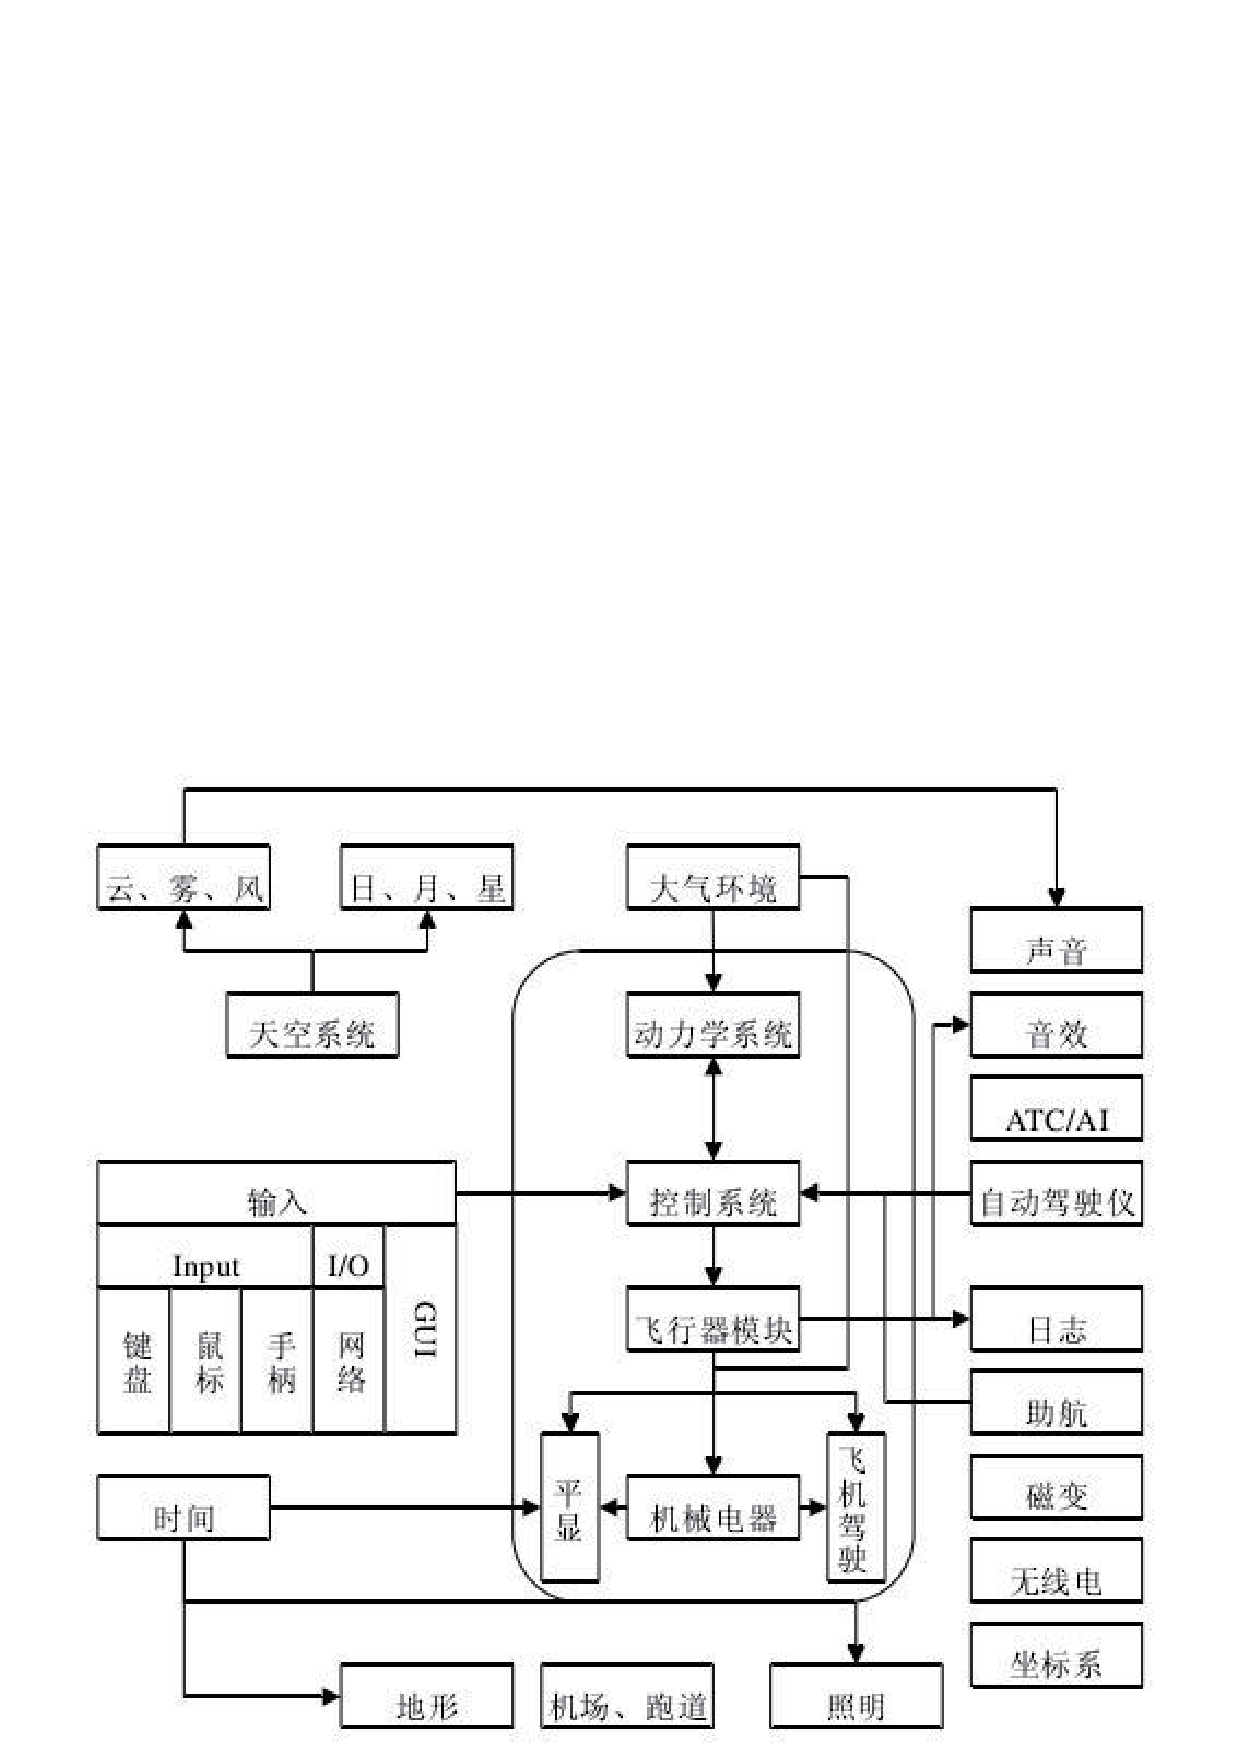
\includegraphics[width=1.0\textwidth]{f15.jpg}
\caption{FlightGear主要组件\ucite{13}}
\label{fig11}
\end{figure}
\subsection{ FlightGear 运行流程}
FlightGear使用C++语言开发,其运行流程如图\ref{fig12}所示\ucite{14}。由图\ref{fig12}可知,FlightGear运行流程主要有两个主循环构成,主循环1 负责完成各个模块的初始化功能。初始化功能通过变量$Idle\_State$累加来控制,随着控制参数$Idle\_State$参数迭代累加的过程,完成各个模块的初始化,主要是助航系统初始化、三维飞行器模型、环境模型(包括天空模型)、OpenGL参数设置,SSG 模块的初始化。同时,主循环1 过程中的窗口系统只要用来完成启动界面的渲染功能。

由图\ref{fig12}可知,在主循环2的过程中,主要完成整个系统更新的功能,是
FlightGear运行过程的核心部分,在该循环过程中的窗口系统则主要用来完成三维化可视仿真系统中的渲染功能\ucite{14},主要针对天空,飞行器,地面等场景的渲染。
\begin{figure}[!ht]
\centering
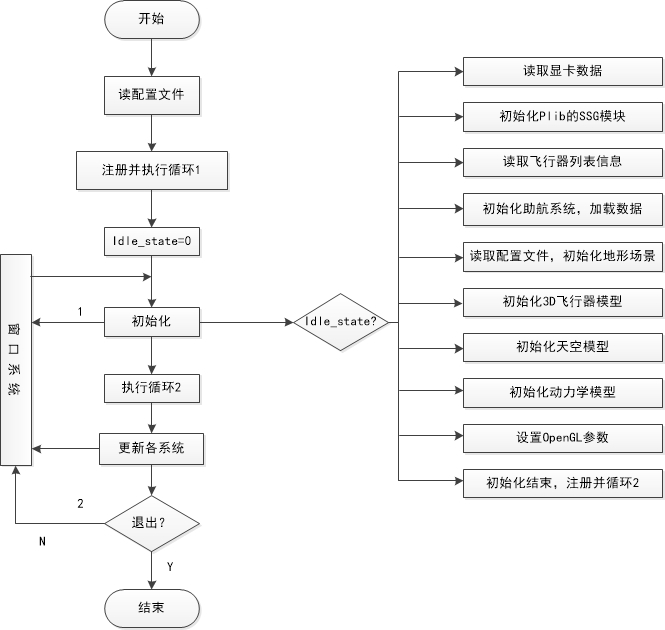
\includegraphics[width=1.0\textwidth]{f16.jpg}
\caption{FlightGear主要组件\ucite{14}}
\label{fig12}
\end{figure}
